\nonstopmode
\documentclass{beamer}
\usepackage{tikz}

\usetikzlibrary{plotmarks}
\usepackage{pgfplots}
\pgfplotsset{compat=1.5}

\usepackage{shellesc}
\usepackage{minted}
\setminted[python]{tabsize=2, linenos=true, breaklines=true}

\usepackage{multirow}
\usepackage{booktabs}
\usepackage{pbox}
\renewcommand{\arraystretch}{1.5}

\usepackage[binary-units]{siunitx}

\usepackage{ulem}

\usepackage{appendixnumberbeamer}

\usepackage{color}
\usepackage{hyperref}

\title{Op zoek naar een goede afstelling van de fiets\\
met een genetisch algoritme}

\author{Michiel Vos}

\date{23 september 2016}

\begin{document}

\begin{frame}
  \titlepage
\end{frame}

\begin{frame}
  \frametitle{Doel}
  \begin{itemize}
      \item Michiel
      \item Theorie
      \item Praktijk (bonus)
  \end{itemize}
\end{frame}

\begin{frame}
  \frametitle{Probleem}
  \begin{itemize}
      \item Fiets 
      \item Veel onderdelen
      \item Optimale afstelling 
  \end{itemize}
\end{frame}

\begin{frame}
  \frametitle{Opties}
  \begin{itemize}
      \item Brute kracht
      \item Gretig algoritme
      \item Genetisch algoritme
  \end{itemize}
\end{frame}

\begin{frame}
  \frametitle{Genetich algoritme}
  \begin{itemize}
      \item Evolutietheorie
      \item Natuur nabootsen
      \item Toepassing op praktisch probleem
      \item Evolutie versnellen
  \end{itemize}
\end{frame}

\begin{frame}
  \frametitle{Onderdelen}
  \begin{center}
    
\includegraphics[width=200px]{michiel.png}
  \end{center}
\end{frame}

\begin{frame}
  \frametitle{Individu}
  \begin{itemize}
      \item Oplossing
      \item DNA
      \item \begin{tabular}{|M | M | M|}
              \hline
              $stuur_0$ $zadel_1$ $verzet_0$ $\dots$ \\ \hline
            \end{tabular}
      \item \begin{tabular}{|M|}
              \hline
              0 1 0 0 1 0 1 0 1 1 1 0 1 \\ \hline
            \end{tabular}
  \end{itemize}
\end{frame}

\begin{frame}
  \frametitle{Fitness}
  \begin{itemize}
      \item Correlatie overlevingskans van genen
      \item Tijdrit vaste omstandigheden
      \item Vaak schatting of simulatie
  \end{itemize}
\end{frame}

\begin{frame}
  \frametitle{Populatie}
  \begin{itemize}
      \item Grootte 
      \item Generatie 0
      \item Willekeur
  \end{itemize}
  \begin{tabular}{|L|M|R|}
    \hline
    Ind. & DNA & Fitness (km/u) \\ \hline
    0 & 1 1 0 1 0 0 0 1 1 1 0 1 &  32 \\ \hline
    1 & 0 1 1 0 0 1 0 1 1 1 0 1 & 53 \\ \hline
    2 & 1 1 0 1 0 1 0 1 0 1 1 1 & 50 \\ \hline
    3 & 1 0 0 1 1 0 0 1 1 0 0 1 & $-5$ \\ \hline
    4 & 0 1 0 1 0 1 1 1 1 1 0 1 & 40 \\ \hline
  \end{tabular}
\end{frame}

\begin{frame}
  \frametitle{Selectie}
  \begin{itemize}
    \item Twee individu\"en
    \item Beste versus willekeur
    \item Voorbeeld roulette selectie:
  \end{itemize}
  \begin{centering}
    \begin{tabular}{|L|M|R|}
      \hline
      Ind. & Fitness (km/u) & Kans \\ \hline
      0 & 32 & $32/(32+53+50) \approx 24\%$ \\ \hline
      1 & 53 & $53/(32+53+50) \approx 39\%$ \\ \hline
      2 & 50 & $50/(32+53+50) \approx 37\%$ \\ \hline
    \end{tabular}
  \end{centering}
\end{frame}

\begin{frame}
  \frametitle{Combinatie}
  \begin{itemize}
    \item Reproductie
    \item Voorbeeld willekeurige combinatie:
  \end{itemize}

  \begin{centering}
      \begin{tabular}{|L|L|M|R|}
        \hline
              Generatie & Ind. & DNA & Fitness (km/u) \\ \hline
              0 & 0 & {\color{red} 1 1 0 1 0 0 0 1 1 1 0 1} &  32 \\ \hline
              0 & 1 & {\color{blue} 0 1 1 0 0 1 0 1 1 1 0 1} & 53 \\ \hline
              1 & 0 & 
                {\color{blue} 0} 
                {\color{blue} 1}
                {\color{red} 0}
                {\color{red} 1}
                {\color{blue} 0}
                {\color{blue} 1}
                {\color{blue} 0}
                {\color{red} 1}
                {\color{red} 1}
                {\color{blue} 1}
                {\color{blue} 0}
                {\color{red} 1}
                & 54 \\ \hline
      \end{tabular}
  \end{centering}
\end{frame}


\begin{frame}
  \frametitle{Mutatie}
  \begin{itemize}
    \item ``Fouten''
    \item Voorbeeld willekeurige mutatie:
  \end{itemize}

  \begin{centering}
      \begin{tabular}{|L|L|M|R|}
        \hline
              Generatie & Ind. & DNA & Fitness (km/u) \\ \hline
              1 & 0 & 
                {\color{blue} 0} 
                {\color{blue} 1}
                {\color{red} 0}
                {\color{red} 1}
                {\color{blue} 0}
                {\color{blue} 1}
                {\color{blue} 0}
                {\color{red} 1}
                {\color{red} 1}
                {\color{blue} 1}
                {\color{blue} 0}
                {\color{green} 0}
                & 54 \\ \hline
      \end{tabular}
  \end{centering}
\end{frame}

\begin{frame}
  \frametitle{Populatie}
  \begin{itemize}
      \item Herhaal selectie, combinatie, mutatie
      \item Generatie 1
      \item Elitisme
      \item Herhaal voor volgende generatie
      \item Stoppen?
  \end{itemize}
\end{frame}

\begin{frame}
  \frametitle{Conclusie}
  \begin{itemize}
      \item Michiel
      \item Natuur inspiratiebron
      \item GA: Balans tussen vrijheid en sturen
      \item Per stap verschillende methodes
      \item Traveling Salesman Problem demo: \url{https://www.youtube.com/watch?v=efTyb82GEDw}
  \end{itemize}
\end{frame}

\begin{frame}
  \frametitle{Vragen?}
  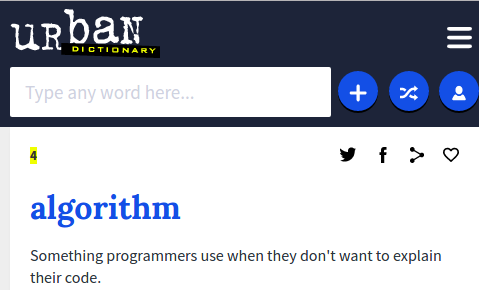
\includegraphics[width=300px]{algorithm.png}
\end{frame}

\end{document}
